\chapter{関連研究}

\section{画像認識における深層学習}
\subsection{概観}
深層学習とは、多層のニューラルネットワークを用いて高い識別性能を達成するモデルを構築する機械学習技術の一つである。
Convolutional Neural Network (CNN)とは、画像認識分野において近年目覚ましい成果を挙げている多層ニューラルネットワークで、
2012年に大規一般画像認識のコンペティションであるILSVRCでCNNを用いたチームが優勝して依頼、画像に関する様々なタスクにおいて利用されている。
従来の画像認識では人手によって画像に有効であると考えられる特徴量を設計し,その特徴量を用いて識別器を学習するというフレームワークであったが、
CNNは、学習の過程で訓練データから識別に有効な特徴量を抽出する表現学習と識別器の学習が同時に行われる点で特徴的である。

しかし一般に、高い汎化性能を持つCNNを学習させるには大量のラベルつきデータセットを構築する必要があるという問題がある。
本節の残りでは、過学習を防ぐために使用されるいくつかの手法について説明する。\todo{ちょっと言い方かえる}

\subsection{Dropout正則化}
一般に機械学習では、訓練データに対する過学習を防ぎ汎化性能を向上させるために、モデルの正則化が行われる。
ニューラルネットワークの正則化手法の一つにDropout\cite{hinton2012improving, srivastava2014dropout}がある。
Dropoutとは、学習の過程において、ニューラルネットワークの中間層のニューロンを一定確率でランダムに"drop"する、すなわち出力を0にする正則化手法である(Fig. \ref{fig:dropout_network})。
これは、任意のn次元中間層の出力に対し、以下のようなマスクをかけることで行われる。\todo{式}
\begin{eqnarray}
    \begin{split}
        y'_i &=& y_i \otimes M \\
        \\
        M &=& [m_0, m_1, \dots, m_n],\;\; m_i \sim Bernoulli(\pi) 
    \end{split}
\end{eqnarray}

% \begin{eqnarray}
%     y'_i &=& y_i \otimes M \\
% % \end{eqnarray} y}
%     M &=& [m_0, m_1, \dots, m_n],\;\; m_i \sim Bernoulli(\pi) 
% \end{eqnarray}

\begin{figure}[tbp]
    \label{fig:dropout_network}
    \begin{minipage}{0.5\hsize}
     \begin{center}
      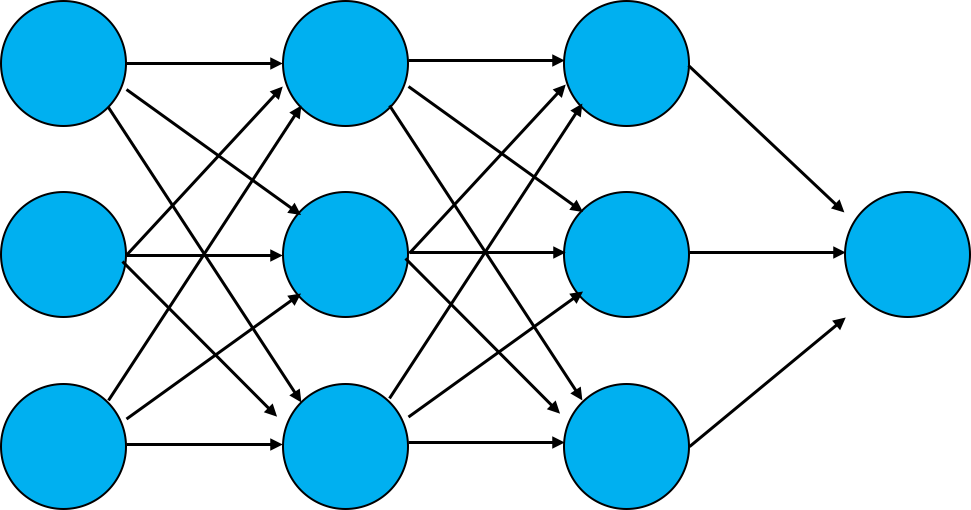
\includegraphics[width=60mm]{figures/standard_network.png}
     \end{center}
     \label{fig:one}
    \end{minipage}
    \begin{minipage}{0.5\hsize}
     \begin{center}
      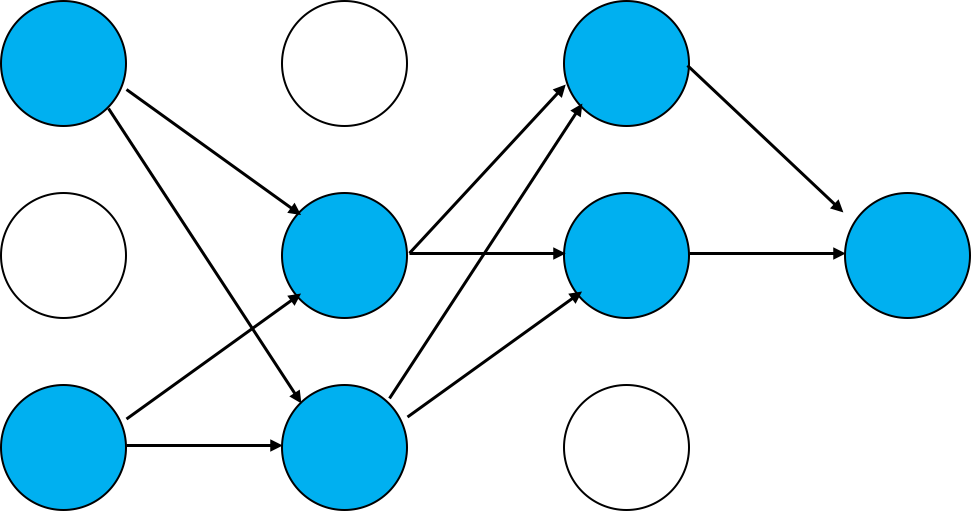
\includegraphics[width=60mm]{figures/dropout_network.png}
     \end{center}
     \label{fig:two}
    \end{minipage}
    \caption{Dropoutの模式図。(左)通常のネットワーク (右)いくつかのニューロンをDropされたネットワーク}
    
\end{figure}

これにより、あるニューロンが特定のニューロンにのみ過剰に依存してしまう共適合(Co-adaptation)を防ぐことができる。
また、指数的な数の部分ネットワークを同時に学習していると見なすこともでき、
複数の部分ネットワークのアンサンブルを行っているのと同じ効果があるとも見なすことが出来る。

\subsection{Data Augmentation}

Data Augmentationとは、画像識別問題においてニューラルネットワークの過学習を防ぐために利用される正則化手法である。
訓練時に、入力された画像に対しラベル情報を保持する程度の変形(幾何学的変形)を加えたものを利用して学習を行うことで、
画像の様々な変形に対し不変な特徴量抽出、及び予測をすることを期待するものである。

例として、モデルに回転不変性を与えるために元画像を回転を加える、位置不変性を与えるために元画像に平行移動を加える等の変形がしばしば用いられる。

\subsection{学習済みモデルからの転移学習}
\label{sec:transfer}
転移学習とは、ある問題を効率的に解くために、別の関連した問題のデータや学習結果を再利用する枠組みである。
深層学習における転移学習とは、しばしばfine-tuningによるものを指すことが多い。
fine-tuningとは、ニューラルネットワークを学習するため、別の問題もしくは別のデータセットで学習済みのモデルを初期値として利用して再学習を行うことである。
これを行うことで、比較的少数の訓練データから優れた性能が得られることが示されている。\todo{引用}

\section{病理画像解析}
本節では、病理画像解析特有の性質と関連研究を述べる。

\subsection{概観}
第1章で述べたように、病理画像とはWSIと呼ばれる巨大なデジタル画像のことを指す。
病理画像解析のおけるアプリケーションは、大きく分けて3つに分類される\cite{komuraishikawa}。
自動診断による医師の補助、類似画像検索による医師の補助、画像と画像以外の情報との関連性の解析、が挙げられる。
近年の画像認識技術の向上による、自動診断に関する研究が急速に増加している。
本研究でも、自動診断に位置づけられる癌の自動検知タスクに焦点を当てる。

\begin{figure}[tbp]
    \label{fig:path_images}
     \begin{center}
      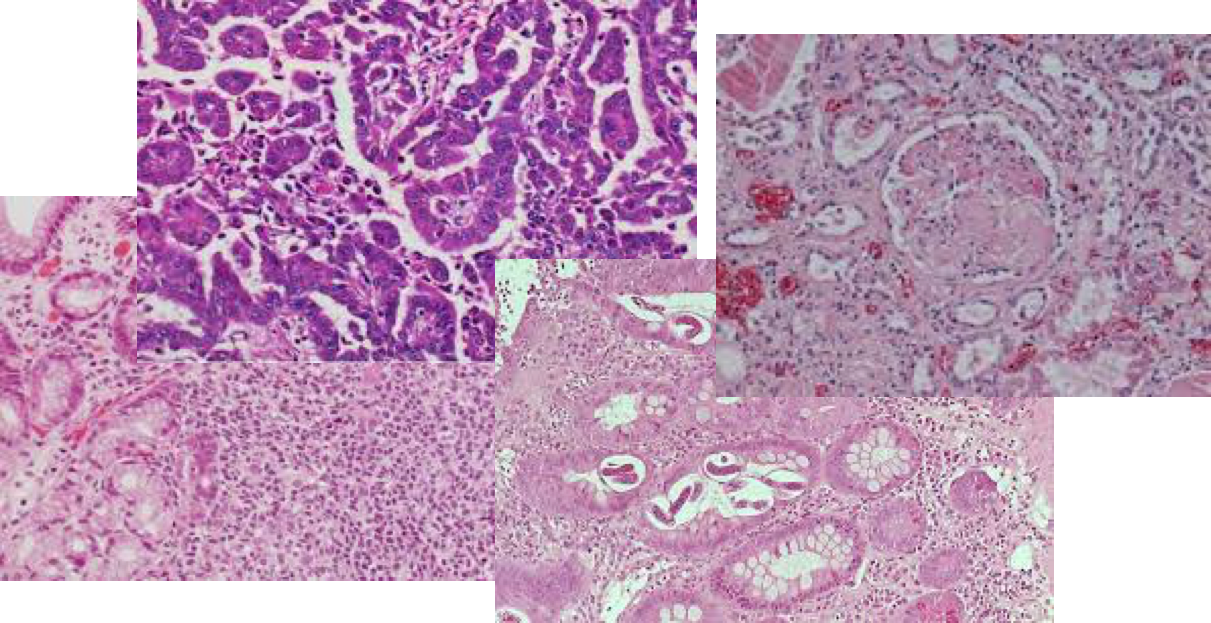
\includegraphics[width=13cm]{figures/path_images.png}
     \end{center}
    \caption{病理画像の例。\todo{もうちょいいい感じのやつ}}
\end{figure}
    
\subsection{WSI全体の予測の出力方法}
一般に、画像認識タスクにおいて用いられる画像はせいぜい1000×1000以下である。
しかし、数万ピクセル×数万ピクセルに及ぶWSIを一度に学習するのはデータ数、パラメータサイズどちらの面においても現実的ではない。
また、癌などの異常部位というのはWSIにおいてわずか領域にのみ現れることも多いため、基本的にはWSIを大量の画像パッチに分割し、
それぞれを識別した結果を統合することで癌の有無を判定することが多い。
個々の画像パッチを識別するのは、SVM, Convolutional Neural Networkなどが用いられる。

\subsection{使用される画像特徴量について}
機械学習において特徴量抽出は重要な役割を持つ。
一般に医療画像解析では、一般画像認識に使用されるSIFT, SURFなどのhand-craftedの画像特徴量が同様に利用されていた。\todo{引用}
また、病理画像はオブジェクトとしての特徴よりもテクスチャとしての性質を持つことから、HLAC, LBPなどのテクスチャ解析における手法が利用されることもあった。\todo{引用}。
ただ、近年では一般画像認識における深層学習の成果を受けて、CNNを利用する研究がほとんどである。
また、多くの医療画像解析ではラベル付きデータが少ないことから、ImageNetなどのデータセットを学習済みのpretrained modelの中間特徴量を特徴量として抽出し識別機はSVMなどを利用する場合と、
\ref{sec:transfer}で述べたような転移学習を利用する場合がある。
一般画像を認識するために学習された特徴量であっても、十分の性能を達成することができることが知られている。\todo{引用}

一般に医療画像解析に共通している特徴として、獲得すべき不変性が多いということがある。
向き、回転不変性、位置不変性、輝度不変性などが一般に用いられる。
また、病理画像では染色液によって細胞を染色することで核などの病理学的特徴を見つけ出すが、その染まり方は細胞毎、研究機関毎に大きく異なる\todo{図があればいいかも}
このことから、強い色相不変性が必要である。

\section{能動学習}

この節では、能動学習について基本的な概念および先行研究について述べる。
また、近年の深層学習を識別器として利用した能動学習や、病理画像解析に能動学習を適用した例についても触れる。

\subsection{基本的な概念}
能動学習,Active Learning\cite{settles2010active}とは,機械学習における一つの枠組みである.
一般に,教師つき学習において識別精度の高いモデルを学習させるためには膨大なラベル付きデータが必要となる.
そこで,能動学習では,得られた大量のラベルなしデータから最もモデル更新に寄与する可能性のあるサンプルを選択し、
それにアノテーションを付与することで,少ないアノテーションコストのもとでいかに高精度な学習モデルを作成するかを目的としている.
データ自体は豊富にあるが、アノテーション付与のコストが高価であるような問題に用いられる。

能動学習の基本的な流れを以下に示す
\begin{description}
    \item[1.] モデル更新に寄与する可能性のあるサンプルを選択 (クエリ問い合わせ)
    \item[2.] 人手,専門家によってアノテーションを付与
    \item[3.] 付与されたアノテーションを利用し教師あり学習を実行
\end{description}
学習が飽和するまでこれらのサイクルを繰り返す。

モデル更新に寄与する可能性があると判断する基準(クエリ選考基準)は様々な側面から提案された手法があり、詳細は後述する。
能動学習全般に当てはまる問題として、学習主体が選択しアノテーションを付与されたデータ集合は、実際のデータ集合とは異なるという問題である。
これをサンプリングバイアスと呼ぶ。

学習主体がクエリを問い合わせる問題設定は以下の3種類に大別される
% \subsubsection{Stream-Based Selective Sampling}
% ストリーミングデータ (サンプルが次々に入力されていくような場合) に対するアプローチ。
% 入力されるストリーミングデータに対してそれぞれのサンプルにラベルを付けるかを逐一判断し,
% モデル更新に寄与すると判断された場合(大抵は閾値を設ける)、クエリとして問い合わせる方式である。
% \subsubsection{Pool-Based Sampling}
% 大量にラベルなしサンプルプールがまとまって与えられている問題に対するアプローチである.
% ストリーミングデータの場合とは違い、閾値を設けることなくプールの中から最もモデル更新に寄与するサンプルを選択することができる。
% また、サンプルデータの分布、およびデータ構造を考慮したクエリ選択が可能となる。
% \subsubsection{Membership Query Synthesis} 
% ストリーミングデータ、プールサンプルどちらの状況でも利用され、
% 実際のデータを直接クエリとして利用するのではなく1つまたは複数のサンプルから新しい人口データを生成し
% 人間に提示する事でラベル付けを行う方法である.
\begin{description}
    \item[Stream-Based Selective Sampling]\mbox{}\\
        ストリーミングデータ (サンプルが次々に入力されていくような場合) に対するアプローチ。
        入力されるストリーミングデータに対してそれぞれのサンプルにラベルを付けるかを逐一判断し,
        モデル更新に寄与すると判断された場合(大抵は閾値を設ける)、クエリとして問い合わせる方式である。
    \item[Pool-Based Sampling]\mbox{}\\
        大量にラベルなしサンプルプールがまとまって与えられている問題に対するアプローチである.
        ストリーミングデータの場合とは違い、閾値を設けることなくプールの中から最もモデル更新に寄与するサンプルを選択することができる。
        また、サンプルデータの分布、およびデータ構造を考慮したクエリ選択が可能となる。
    \item[Membership Query Synthesis]\mbox{}\\ 
        ストリーミングデータ、プールサンプルどちらの状況でも利用され、
        実際のデータを直接クエリとして利用するのではなく1つまたは複数のサンプルから新しい人口データを生成し
        人間に提示する事でラベル付けを行う方法である.
\end{description}

中でも、Pool-based Samplingの問題設定での研究が最も行われており、本研究でも大量のラベルなし病理画像データプールは予め与えられているものとする。

\subsection{クエリ選考基準}
\label{query_strategy}
本項では、モデル更新に寄与する可能性が高いと判断するためのクエリ選考基準として提案されているいくつかのものについて述べる

$\mathcal{L}$をラベル付きデータセット、$\mathcal{U}$をラベルなしデータセットとする

\subsubsection{Uncertainty Sampling}
最もシンプルな戦略で、モデルが自身の予測が最も曖昧であるようなサンプルをクエリとして選択する。
データ$x$が与えられた時、ラベルの確率分布$p(y|x)$を出力する識別器を用いれば利用することが出来るため、幅広く利用されている。
曖昧であることの定量評価として、事後確率最大ラベルの確率が小さいサンプルを選択するLeast Confident、事後確率最大ラベルの確率と、
その次に大きなラベルの確率との差が小さいサンプルを選択するMargin Sampling、事後確率分布のエントロピーが大きいサンプルを選択するEntropy Samplingなどが提案されている。
これらは、二値分類の場合は全て等価な戦略となる。
% Least Confident : 最も事後確率が高いクラスラベルの予測確率が最も小さくなるものを選ぶ
% \begin{equation}
%     x^{*} = \argmax_x \: 1 - P_{\theta}(\hat{y}|x)
% \end{equation}

\subsubsection{Query By Committee}
モデルのバージョン空間 (モデルの仮説空間内で現在のラベル付きデータに対してConsistentな領域)を
縮小させるサンプルが更新に寄与するはずだとする仮説に基づく戦略。
実際にバージョン空間をすべて保持することは現実的には不可能であるため、近似的にこれを扱うための手法の一つがQuery-By-Committee (QBC)\cite{seung1992query}アルゴリズムである。
バージョン空間を近似的に表現するために、現在のラベル付きデータ集合から学習された
複数のモデル(committee $C=\{ \theta^{(1)}, \dots, \theta^{(C)}\}$)を保持し、
それぞれのcommitteeの予測が最も不一致するサンプルを選択するという戦略である。
不一致度の定量評価として、Vote Entropy、Average Kullback Divergenceがある。
Vote Entropyは、それぞれのcommitteeがどのラベルだと予測(投票)したかのばらつきを定量化したもので、次式で表される
\begin{equation}
    x^{*} = \argmax_x \: - \sum_i \frac{V(y_i)}{C} \log \, \frac{V(y_i)}{C}
\end{equation}
$V(y_i)$はcommitteeの投票数、$C$はcommitteeのサイズである。

Average Kullback Divergenceは、それぞれ予測分布の確率分布の差異が平均的に大きいものを選ぶ手法である。
\begin{equation}
    x^{*} = \argmax_x \:  \frac{1}{C} \sum_{c=i}^C KL \, (P_{\theta^{(c)}} || P_C)
\end{equation}
$P_C$はcommittee全体の平均の確率予測分布である。

\subsubsection{Expected Model Change / Expected Error Reduction}
データにあるラベルがつけられた場合に、モデルが実際にどう更新されるかの期待値を求めることで、最善のサンプルを選択することができると考えられる。
このような考えに基づき、可能性のあるラベルを全通り試すことでモデルの更新量が最大となるサンプルを選択するのがExpected Model Changeと呼ばれる戦略で、
また、モデルの更新量ではなくモデルの汎化誤差の減少量を評価することを目的とした戦略がExpected Model Changeである。
多くのケースでは、全サンプルのラベルを全通り仮定し、モデルの再学習を行う必要があるため膨大な計算コストを要する手法である。

\subsubsection{Variance Reduction}
モデルの期待汎化誤差は以下のように分解することが出来る。
\begin{equation}
    E_T [(\hat{y} - y)^2|x] = E_T [(y - E[y|x])^2] + (E_{\mathcal{L}}[\hat{y}] - E[y|x])^2 + E_{\mathcal{L}} [(\hat{y} - E_{\mathcal{L}}[\hat{y}^2]
\end{equation}
$E_{\mathcal{L}}[\cdot]$はラベルセット$\mathcal{L}$に関する期待値、$E[\cdot]$は条件付き分布$P(y|x)$に関する期待値、$E_T$はそれぞれに関する期待値である。
上記の右辺は、一項目から、ラベルノイズに関する項、モデルバイアスに関する項、モデルの分散に関する項を表している。
これらのうち、学習によって変更できるのはモデルの分散のみである。
そこで、モデルのパラメータの期待分散を小さくすることで、間接的にモデルの汎化誤差を小さくする戦略がVariance Reductionである。
また、パラメータの分散はフィッシャー情報量$I(\theta)$の逆数によって下界を決定されるという統計的性質から、
モデルのパラメータのフィッシャー情報量を最大化する(もしくは逆数を最小化する)サンプルを選択する問題に帰着される。

\subsubsection{Density Weighted Method}
これまでの戦略とは異なり、単一のサンプルのみを評価するのではなく、周囲のサンプル、もしくは分布全体の構造を考慮する手法である。
周囲にサンプルが多数ある場合と周囲にサンプルが存在しない場合を考慮すると、後者は外れ値のサンプルである可能性が高く前者のほうが
選択する価値が高いと考えられる。
そのような手法の一つにInformation Densityがある。
基本的に、他の選択戦略と併せて使用される手法で、各定量評価に類似度を考慮した係数を掛け合わせることで重みをつける手法である。
\begin{equation}
    x^{*} = \argmax_x \:  \phi(x) \times (\frac{1}{U} \sum_{u=1}^{U} s(x, x_i)))^{\beta}
\end{equation}

$\phi(x)$は他の選択戦略による評価である。$s(\cdot)$はサンプル間の類似度を算出する関数である。

\subsection{関連する他の手法}

\subsubsection{バッチ型能動学習}
多くの能動学習の研究では、クエリ問い合わせは一つのサンプルにのみ行われる。
しかし、近年の機械学習アルゴリズムは計算コストが非常に大きいため、一度に複数のクエリ集合$\mathcal{Q}$を問い合わせるバッチ能動学習に関する研究が増加しつつある。
最もナイーブに考えた場合、\ref{query_strategy}で述べたような定量指標で上から$\mathcal{Q}$個のサンプルを選んだ場合、それらのサンプルには重複した情報が含まれる可能性が高い。
brinker et al.、Xu et al.らはクラスタリング手法によって同一クラスター内からはクエリを選択しないという戦略を提案した\cite{brinker2003incorporating}、\cite{Xu2007}。
また、ChenとKrauseらは、バッチ能動学習を劣モジュラ最適化問題に帰着させることで、貪欲法によって最適な組み合わせと比較した場合の$1 - \frac{1}{e}$近似が可能であることを示した。
\cite{chen2013near}


\section{関連する先行研究と本研究の位置づけ}

\subsection{能動学習の病理分野への適用}
\com{active + Pathology}
能動学習を病理画像解析に利用した研究は複数存在する。
複数人のWSIから切り出したパッチベースでの学習を行う病理画像解析では、クエリとしてWSI中の1領域を問い合わせるのが自然である。
しかし、通常のデータ分布とは違い、独立同一分布 (i.i.d)でない特徴がある。
NalisNik et al.はUncertainty Samplingによる能動学習を比較的単純な細胞核segmentationタスクに応用した\cite{nalisnik2017interactive}。
class balancing + query-by-committee\cite{doyle2011active}, 
logistic regression + variance reduction \cite{padmanabhan2014active},
仮説空間の縮小を目的関数にすることで劣モジュラ最適化の枠組みを利用、似たデータが多いことを利用してk-meansでクラスタリング\cite{zhu2014scalable}、
しかし、そのほとんどが人手によって設計された特徴量に対して線形の識別器を用いているものであるため、精度の点で十分であるとは言えない。

\subsection{深層能動学習}
能動学習の研究は、理論、実践的なアプリケーションどちらも線形識別器を用いているものが大半であるが、
近年の深層学習の成果を受けて、深層学習と能動学習を組み合わせた研究も行われている\cite{6889457, li2016active}。
これらのアプローチは、Restricted Boltzmann Machinesやstacked autoencodersなどによってpre-trainingを行ったネットワークを用いて、
Uncertainty Samplingによるクエリ選択を行うというシンプルなものである。\todo{もうちょいかく}

\subsection{本研究の位置づけ}
能動学習において深層学習を利用する研究の多くは、Uncertainty Samplingベースのクエリ選考基準を用いている。
これらのアプローチでは、多層ニューラルネットワークの予測の不確かさを定量的に評価するために、出力の確率分布のエントロピーが大きさなどが利用されることが多い。
しかし、一般に、多層ニューラルネットワークは自らの予測に対する不確かさを陽に表すようにモデル化されていない。
仮に予測が0.9という高い確率であったとしても、確信度が高いことを示すわけではないという問題がある。\todo{非線形だからどこで間違ってるかわからん。}
\todo{ベイスCNN触れる}

本研究では、不確かさを陽にモデル化しない多層ニューラルネットワークを能動学習に効率的に組み込むために手法を提案し、
精度を犠牲にすることなく、安定してアノテーションコストを削減する病理画像解析システムを提案する。
多層ニューラルネットワークにとってモデル更新に寄与すると考えられるサンプルを選択するために、Query-By-Committeeのアイデアを基に
DropoutとData Augmentationを推論にも利用することにより近似的にそれらを達成するアプローチを取る。

\section{まとめ}
本章では、本研究に関連するいくつかの研究の枠組みと、先行研究について述べた。
また、その中での本研究の位置づけを述べた。
次の章では、具体的に本研究で提案するシステムを説明する。